%%%%%%%%%%%%%%%%%%%%%%%%%%%%%%%%%%%%%%%%%
% Beamer Presentation
% LaTeX Template
% Version 1.0 (10/11/12)
%
% This template has been downloaded from:
% http://www.LaTeXTemplates.com
%
% License:
% CC BY-NC-SA 3.0 (http://creativecommons.org/licenses/by-nc-sa/3.0/)
%
%%%%%%%%%%%%%%%%%%%%%%%%%%%%%%%%%%%%%%%%%

%----------------------------------------------------------------------------------------
%	PACKAGES AND THEMES
%----------------------------------------------------------------------------------------

\documentclass{beamer}

\mode<presentation> {

% The Beamer class comes with a number of default slide themes
% which change the colors and layouts of slides. Below this is a list
% of all the themes, uncomment each in turn to see what they look like.

%\usetheme{default}
%\usetheme{AnnArbor}
%\usetheme{Antibes}
%\usetheme{Bergen}
%\usetheme{Berkeley}
%\usetheme{Berlin}
%\usetheme{Boadilla}
%\usetheme{CambridgeUS}
%\usetheme{Copenhagen}
%\usetheme{Darmstadt}
%\usetheme{Dresden}
%\usetheme{Frankfurt}
%\usetheme{Goettingen}
%\usetheme{Hannover}
%\usetheme{Ilmenau}
%\usetheme{JuanLesPins}
%\usetheme{Luebeck}
\usetheme{Madrid}
%\usetheme{Malmoe}
%\usetheme{Marburg}
%\usetheme{Montpellier}
%\usetheme{PaloAlto}
%\usetheme{Pittsburgh}
%\usetheme{Rochester}
%\usetheme{Singapore}
%\usetheme{Szeged}
%\usetheme{Warsaw}

% As well as themes, the Beamer class has a number of color themes
% for any slide theme. Uncomment each of these in turn to see how it
% changes the colors of your current slide theme.

%\usecolortheme{albatross}
%\usecolortheme{beaver}
%\usecolortheme{beetle}
%\usecolortheme{crane}
%\usecolortheme{dolphin}
%\usecolortheme{dove}
%\usecolortheme{fly}
%\usecolortheme{lily}
%\usecolortheme{orchid}
%\usecolortheme{rose}
%\usecolortheme{seagull}
%\usecolortheme{seahorse}
%\usecolortheme{whale}
%\usecolortheme{wolverine}

%\setbeamertemplate{footline} % To remove the footer line in all slides uncomment this line
%\setbeamertemplate{footline}[page number] % To replace the footer line in all slides with a simple slide count uncomment this line

%\setbeamertemplate{navigation symbols}{} % To remove the navigation symbols from the bottom of all slides uncomment this line
}

\usepackage{graphicx} % Allows including images
\usepackage[absolute, overlay]{textpos}
\usepackage{booktabs} % Allows the use of \toprule, \midrule and \bottomrule in tables
\usepackage{tikz}
\usetikzlibrary{positioning,calc,shapes.callouts,shapes.arrows}

\tikzset{My Arrow Style/.style={single arrow, fill=red!30, anchor=base, align=center,text width=2.8cm}}
\newcommand{\arrowthis}[2][]{\tikz[baseline] \node [My Arrow Style,#1] {#2};}


\tikzset{My Speech Style/.style={ellipse callout, fill=red!50, anchor=base, align=center,text width=2.8cm}}
\newcommand{\speechthis}[2][]{
    \tikz[baseline]{\node[My Speech Style, #1]{#2};}
}%

%----------------------------------------------------------------------------------------
%	TITLE PAGE
%----------------------------------------------------------------------------------------

\title[University of Bucharest]{An Immediate Multi-Party Generalization of ID-NIKE from Constrained PRF}
% The short title appears at the bottom of every slide, the full title is only on the title page
%An Immediate Multi-Party Generalization of ID-NIKE from Constrained PRF
\author{Ruxandra F. Olimid, Dragos Alin Rotaru} % Your name
\institute[] % Your institution as it will appear on the bottom of every slide, may be shorthand to save space
{
University of Bucharest\\ % Your institution for the title page
% \medskip
% \textit{ruxandra.olimid@fmi.unibuc.ro, r.dragos0@gmail.com} % Your email address
}
\date{\today} % Date, can be changed to a custom date

\begin{document}

\begin{frame}
\titlepage % Print the title page as the first slide
\end{frame}


%----------------------------------------------------------------------------------------
%	PRESENTATION SLIDES
%----------------------------------------------------------------------------------------

%------------------------------------------------
\section{Overview} % Sections can be created in order to organize your presentation into discrete blocks, all sections and subsections are automatically printed in the table of contents as an overview of the talk
%------------------------------------------------

\begin{frame}
    \frametitle{Asymmetric Crypto Overview} % Table of contents slide, comment this block out to remove it

    \begin{textblock*}{5cm}(0cm, 3cm)
        \begin{figure}
            
\includegraphics[width=5cm,height=3cm,keepaspectratio]{bob.jpg}
            \caption{Bob $sk_1$}
        \end{figure}
    \end{textblock*}

    \begin{textblock*}{2cm}(5.5cm, 1cm)
        \begin{figure}
            
\includegraphics[width=1cm,height=1cm]{eve.png}
            \caption{Eve}
        \end{figure}
    \end{textblock*}

    \begin{textblock*}{5cm}(8cm, 3cm)
        \begin{figure}
            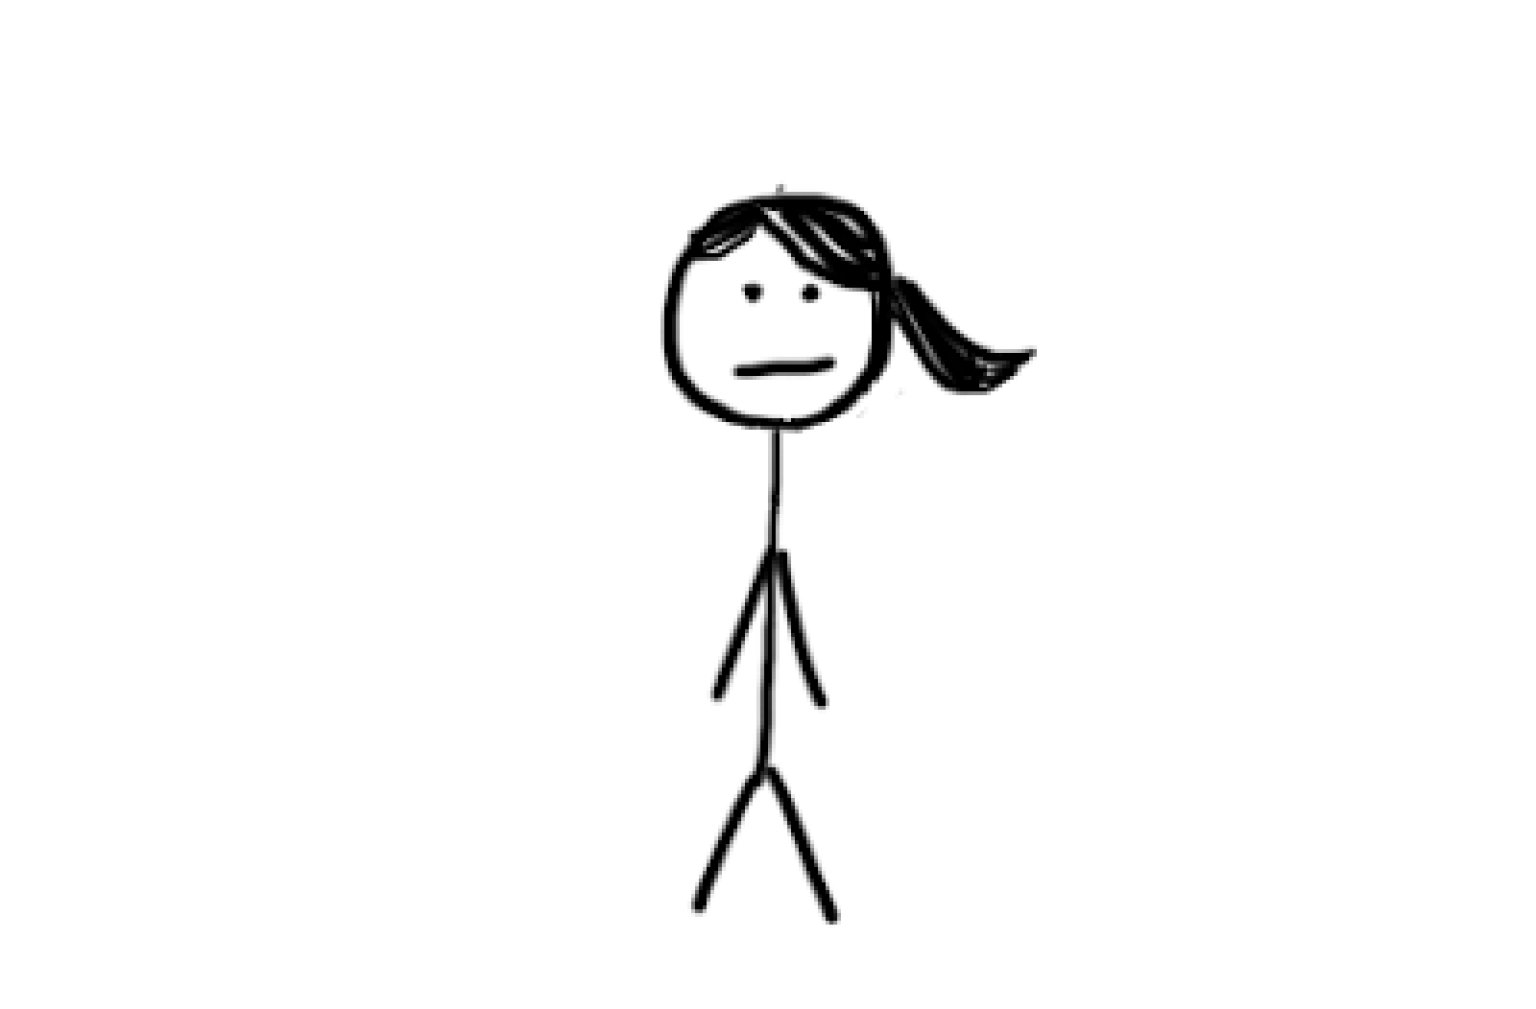
\includegraphics[width=5cm,height=3cm,keepaspectratio]{alice.jpeg}
            \caption{Alice $sk_2$}
        \end{figure}
    \end{textblock*}

    \begin{textblock*}{3cm}(5cm, 5cm)
        \only<2-4>{\arrowthis[]{$c_1 \leftarrow E(pk1, m_1)$}}
    \end{textblock*}

    \begin{textblock*}{3cm}(8cm, 2cm)
        \only<3-4>{\speechthis{I know the message!}}
    \end{textblock*}

    %decription for Alice
    \begin{textblock*}{4cm}(9.5cm, 8cm)
        \only<4->{$m_1 = D(sk_2, c_1)$}
    \end{textblock*}

    %decription for Bob
    \begin{textblock*}{4cm}(1cm, 8cm)
        \only<5->{$m_2 = D(sk_1, c_2)$}
    \end{textblock*}

    %message for Bob
    \begin{textblock*}{3cm}(5cm, 5cm)
        \only<5>{\arrowthis[shape border rotate=180]{$c_2 \leftarrow E(pk2, m_2)$}}
    \end{textblock*}

    %speech for Eve
    \begin{textblock*}{0.5cm}(7cm, 1cm)
        \only<6>{\scalebox{10}{\textbf{?}}}
    \end{textblock*}

\end{frame}

%------------------------------------------------

\begin{frame}
\frametitle{Bullet Points}
\begin{itemize}
\item Lorem ipsum dolor sit amet, consectetur adipiscing elit
\item Aliquam blandit faucibus nisi, sit amet dapibus enim tempus eu
\item Nulla commodo, erat quis gravida posuere, elit lacus lobortis est, quis porttitor odio mauris at libero
\item Nam cursus est eget velit posuere pellentesque
\item Vestibulum faucibus velit a augue condimentum quis convallis nulla gravida
\end{itemize}
\end{frame}

%------------------------------------------------

\begin{frame}
\frametitle{Blocks of Highlighted Text}
\begin{block}{Block 1}
Lorem ipsum dolor sit amet, consectetur adipiscing elit. Integer lectus nisl, ultricies in feugiat rutrum, porttitor sit amet augue. Aliquam ut tortor mauris. Sed volutpat ante purus, quis accumsan dolor.
\end{block}

\begin{block}{Block 2}
Pellentesque sed tellus purus. Class aptent taciti sociosqu ad litora torquent per conubia nostra, per inceptos himenaeos. Vestibulum quis magna at risus dictum tempor eu vitae velit.
\end{block}

\begin{block}{Block 3}
Suspendisse tincidunt sagittis gravida. Curabitur condimentum, enim sed venenatis rutrum, ipsum neque consectetur orci, sed blandit justo nisi ac lacus.
\end{block}
\end{frame}

%------------------------------------------------

\begin{frame}
\frametitle{Multiple Columns}
\begin{columns}[c] % The "c" option specifies centered vertical alignment while the "t" option is used for top vertical alignment

\column{.45\textwidth} % Left column and width
\textbf{Heading}
\begin{enumerate}
\item Statement
\item Explanation
\item Example
\end{enumerate}

\column{.5\textwidth} % Right column and width
Lorem ipsum dolor sit amet, consectetur adipiscing elit. Integer lectus nisl, ultricies in feugiat rutrum, porttitor sit amet augue. Aliquam ut tortor mauris. Sed volutpat ante purus, quis accumsan dolor.

\end{columns}
\end{frame}

%------------------------------------------------
\section{Constrained PRF framework}
%------------------------------------------------

\begin{frame}
\frametitle{References}
\footnotesize{
\begin{thebibliography}{99} % Beamer does not support BibTeX so references must be inserted manually as below
\bibitem[Smith, 2012]{p1} John Smith (2012)
\newblock Title of the publication
\newblock \emph{Journal Name} 12(3), 45 -- 678.
\end{thebibliography}
}
\end{frame}


%------------------------------------------------
\section{Boneh-Waters ID NIKE construction & Our generalization}

%------------------------------------------------

\begin{frame}
\Huge{\centerline{The End}}
\end{frame}


\section{cPRF construction}
%----------------------------------------------------------------------------------------

\end{document}
